\documentclass[tikz, border=2pt]{standalone}

\usepackage{helvet}
\renewcommand{\familydefault}{\sfdefault}

\usepackage[EULERGREEK]{sansmath}
\sansmath
\usetikzlibrary{arrows.meta}
\usetikzlibrary{bending}

\usetikzlibrary{arrows,positioning}
\tikzset{
  shift left/.style ={commutative diagrams/shift left={#1}},
  shift right/.style={commutative diagrams/shift right={#1}}
}


\begin{document}%
\definecolor{liblu}{rgb}{.522, .796, .980}
\definecolor{ligre}{rgb}{.502, .941, .667}

\definecolor{spec1}{rgb}{0.9515524824536824, 0.9411914096412802, 0.942275630291603} 
\definecolor{spec2}{rgb}{0.920542265962946, 0.7739664017130241, 0.8159465662332823}
\definecolor{spec3}{rgb}{0.8895320494722094, 0.6067413937847681, 0.6896175021749618}
\definecolor{spec4}{rgb}{0.858521832981473, 0.4395163858565121, 0.5632884381166412}
\definecolor{spec5}{rgb}{0.8275116164907365, 0.272291377928256, 0.4369593740583205}
\definecolor{spec6}{rgb}{0.7965014, 0.10506637, 0.31063031}


\definecolor{gold}{rgb}{1.0, 0.85, 0.0}

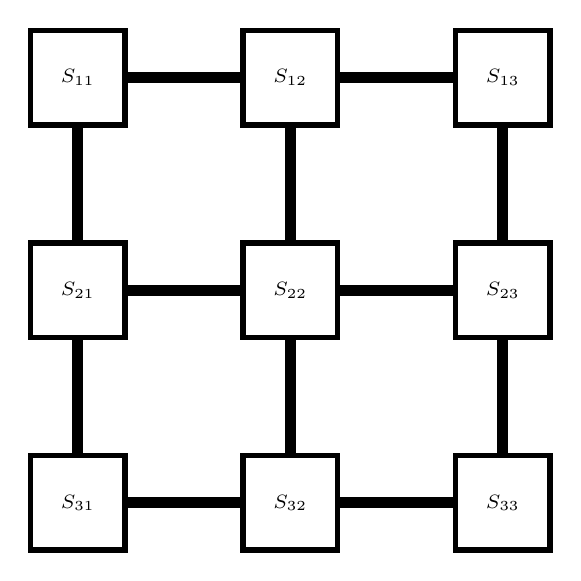
\begin{tikzpicture}[line width=2pt]
\tikzset{>={Latex[width=3mm,length=4mm]}}


% % grid
% \draw[help lines] (-0.5, -8) grid (16.5, 10);

% 3 
\node [rectangle, draw,  fill=white, minimum size=1.2cm] at (1, 8) (a) {\scriptsize $S_{11}$};

\node [rectangle, draw, fill=white, minimum size=1.2cm] at (1 + 2.7, 8) (b) {\scriptsize $S_{12}$};

\node [rectangle, draw, fill=white, minimum size=1.2cm] at (1 + 2*2.7, 8) (c) {\scriptsize $S_{13}$};


\node [rectangle, draw,  fill=white, minimum size=1.2cm] at (1, 8 - 2.7) (a1) {\scriptsize $S_{21}$};

\node [rectangle, draw, fill=white, minimum size=1.2cm] at (1 + 2.7, 8 - 2.7) (b1) {\scriptsize $S_{22}$};

\node [rectangle, draw, fill=white, minimum size=1.2cm] at (1 + 2*2.7, 8 - 2.7) (c1) {\scriptsize $S_{23}$};

\node [rectangle, draw,  fill=white, minimum size=1.2cm] at (1, 5.3-2.7) (a2) {\scriptsize $S_{31}$};

\node [rectangle, draw, fill=white, minimum size=1.2cm] at (1 + 2.7, 5.3-2.7) (b2) {\scriptsize $S_{32}$};

\node [rectangle, draw, fill=white, minimum size=1.2cm] at (1 + 2*2.7, 5.3-2.7) (c2) {\scriptsize $S_{33}$};


\draw [-, draw=black, line width=4pt] (a) -- (b) node[pos=0.5, sloped, above] {};

\draw [-, draw=black, line width=4pt] (b) -- (c) node[pos=0.5, sloped, above] {};

\draw [-, draw=black, line width=4pt] (a) -- (a1) node[pos=0.5, sloped, above] {};

\draw [-, draw=black, line width=4pt] (b) -- (b1) node[pos=0.5, sloped, above] {};

\draw [-, draw=black, line width=4pt] (c) -- (c1) node[pos=0.5, sloped, above] {};
\draw [-, draw=black, line width=4pt] (a1) -- (a2) node[pos=0.5, sloped, above] {};

\draw [-, draw=black, line width=4pt] (b1) -- (b2) node[pos=0.5, sloped, above] {};

\draw [-, draw=black, line width=4pt] (c1) -- (c2) node[pos=0.5, sloped, above] {};

\draw [-, draw=black, line width=4pt] (a1) -- (b1) node[pos=0.5, sloped, above] {};

\draw [-, draw=black, line width=4pt] (b1) -- (c1) node[pos=0.5, sloped, above] {};
\draw [-, draw=black, line width=4pt] (a2) -- (b2) node[pos=0.5, sloped, above] {};

\draw [-, draw=black, line width=4pt] (b2) -- (c2) node[pos=0.5, sloped, above] {};

% \draw [-, draw=black, line width=4pt] (a) -- (b1) node[pos=0.5, sloped, above] {};

% \draw [-, draw=black, line width=4pt] (b1) -- (c) node[pos=0.5, sloped, above] {};
% \draw [-, draw=black, line width=4pt] (a2) -- (b1) node[pos=0.5, sloped, above] {};

% \draw [-, draw=black, line width=4pt] (b1) -- (c2) node[pos=0.5, sloped, above] {};


\end{tikzpicture}


\end{document}